% presentation
\documentclass{beamer}

\usetheme{Warsaw}

% rus lang
\usepackage[main=russian,english]{babel}

% insert images
\usepackage{wrapfig}
\usepackage{graphicx}
\graphicspath{{./img/}}

% declare operator
\DeclareMathOperator*{\argmin}{argmin} % thin space, limits underneath in displays
\newcommand{\at}[2][]{#1|_{#2}}

% math
\newtheorem{rustheorem}{Теорема}
\usepackage{amsmath}
\DeclareMathOperator{\sign}{sign}
\DeclareMathOperator{\K}{K}
\DeclareMathOperator{\R}{\mathbb{R}}
\DeclareMathOperator{\X}{\mathbb{X}}
\DeclareMathOperator{\Y}{\mathbb{Y}}

\title[Деревья решений]{Лекция 6. Деревья решений}
\subtitle{Основы интеллектуального анализа данных}
\author{Полузёров Т. Д.}
\institute{БГУ ФПМИ}
\date{}

\begin{document}
	
	\begin{frame}
		\titlepage
	\end{frame}
	
	
	\begin{center}
		\frametitle{Структура лекции}
		\tableofcontents	
	\end{center}
    
	\section{Понятие решающего дерева}

	\begin{frame}
		\frametitle{Пример дерева решений}
		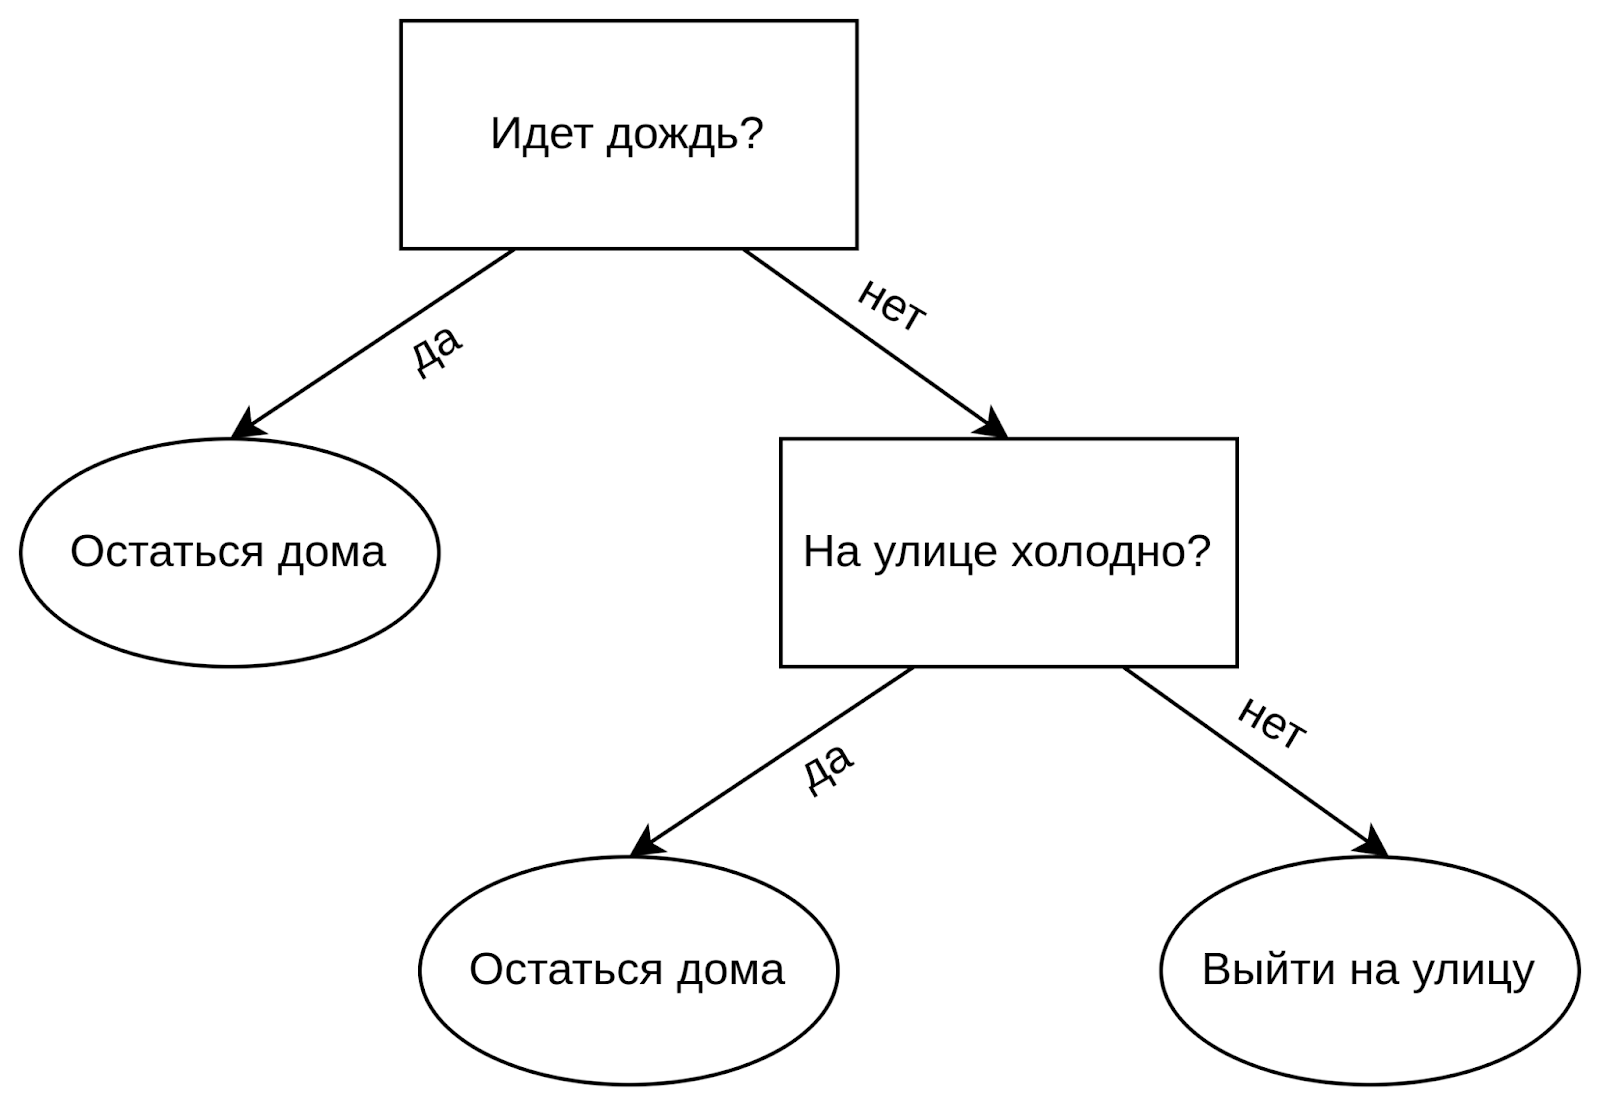
\includegraphics[width=1\textwidth]{dc}
	\end{frame}

    \begin{frame}
        \frametitle{Компоненты бинарного дерева}

		Дерево состоит из 2-х типов вершин:
		\begin{itemize}
			\item \textbf{Внутрення} вершина $v$ хранит в себе предикат $b_v: \X \rightarrow \{0, 1\}$
			\item \textbf{Листовая вершина} $v$ хранит выходное значение $c_v \in \Y$
		\end{itemize}

		\vspace{15pt}

		Любая внутрення вершина имеет ровно двух потомков.

		Любая листовая вершина не имеет потомков.

		\vspace{15pt}

		\textbf{Глубина дерева} $h$ --- длина наибольшего маршрута от корня до листа.
    \end{frame}
	
	\begin{frame}
		\frametitle{Алгоритм работы дерева}

		Алгоритм $a(x)$ работает по схеме:
		\begin{enumerate}
			\item Стартуем из корня
			\item Вычисляем предикат в текущей вершине
			\item Если $b_v = 1$ - шагаем в право, $b_v = 0$ - в лево
			\item Пока не дошли до листовой вершини, повторяем с шага 2
			\item Возвращаем значение в листе $c_v$
		\end{enumerate}
	\end{frame}

	\begin{frame}
		\frametitle{Голосование конъюнкций}
	
		Объект $x$ доходит до листовой вершины $v$ тогда и только тогда, когда выполняется конъюнкция
		$K_v(x)$ всех предикатов на пути от корня до $v$.

		\vspace{15pt}

		$T$ --- множество листовых вершин. 
		
		$A_v = \{x \in X | K_v(x) = 1), v \in T\}$ --- множества выделяемые конъюнкциями.
		Причем эти множества не пересекаются, а в объединении совпадают с $X$.
		
		\vspace{15pt}

		Решающее дерево как алгоритм классификации:
		\[
		a(x) = \arg \max_{y \in Y} \sum_{v \in T} [c_v = y] K_v(x)
		\]
		причем при любом $x$ только одно слагаемое равно единице.
	\end{frame}

	\begin{frame}
		\frametitle{Предикаты}

		Предикат - любая решащая функция $b :\X \rightarrow \{0, 1\}$
		
		\vspace{15pt}

		\begin{itemize}
			\item Пороговая функция $b(x) = [x_i > t]$
			\item Линейный $b(x) = [\langle x, \omega \rangle > t]$
			\item Метрический $b(x) = [\rho(x, x_v) > t]$, где $x_v$ - некоторый объект выборки
		\end{itemize}

		\vspace{15pt}

		Но выбор сложных предикатов - излишен. Поэтому используются $b(x) = [x_i > t]$
	\end{frame}

	\begin{frame}
		\frametitle{Свойства дерева}
		
		После определения дерева видно несколько свойств:
		\begin{itemize}
			\item Дерево есть набор из $|T|$ конъюнкий, непересекающихся и покрывающих все пространство $X$.
			\item Алгоритм $a(x)$ --- кусочно постоянная функция.Градиентные методы не применимы.
			\item Дерево способно полностью выучить обучающую выборку. В этом случае низкая обобщаяющая способность.
		\end{itemize}
	\end{frame}

	\section{Построение дерева}

	\subsection{Решающий пень}

	\begin{frame}
		\frametitle{Решающий пень}
		Пусть имеется размеченная выборка $X = (x_1, \dots x_{\ell}), x_i \in \R^n, Y = (y_1, ..., y_{\ell})$.

		\vspace{15pt}

		Необходимо минимизировать функцию качества $L(X)$.
		Используя предикат $b(x_i| j, t) = [x_i^j > t], j=1, \dots, n$ хотим~разбить $X = X_L \cup X_R$, чтобы

		$L(X) > L(X_L) + L(X_R)$

		\vspace{15pt}

		И даже 

		\[
		j^*, t^* = \arg \min L(X_L) + L(X_R)
		\]
	\end{frame}

	\begin{frame}
		\frametitle{Сложность построения}

		Для вычисления предиката $b(x)$ по выборке необходимо $O(\ell)$.

		А для перебора всевозможных пар $(j, t)$ потребуется $O(\ell n)$.

		И итоговая сложность построения пня есть $O(\ell^2 n)$.

		\vspace{15pt}

		Если строить дерево произвольной глубины на котором достигается минимум на тестовой выборке 
		--- задача становится NP-полной.
		Поэтому разрешим себе строить не оптимальные, но хорошие деревья.
	\end{frame}

	\subsection{Жадный алгоритм}

	\begin{frame}
		\frametitle{Жадный алгоритм}

		Очевидной идеей есть строить дерево рекурсивно, как для случая решающего пня.

		\vspace{15pt}

		Алгоритм :

		На входе имеется выборка $X_m$
		\begin{enumerate}
			\item Создать вершину $v$
			\item Если выполнен критерий остановки $Stop(X_m)$ --- делаем $v$ листом и приписываем ответ $Ans(X_m)$
			\item Иначе, перебираем предикаты и находим $(i^*, j^*)$ который производит разбиение $X = X_L \cup X_R$ максимизируя
			критерий ветвления $Branch(X_m, i, j)$
			\item Вызвать рекурсивно для $X_L$ и $X_R$ эту процедуру
		\end{enumerate}
	\end{frame}

	\begin{frame}
		\frametitle{Неоптимальность жадного алгоритма}

		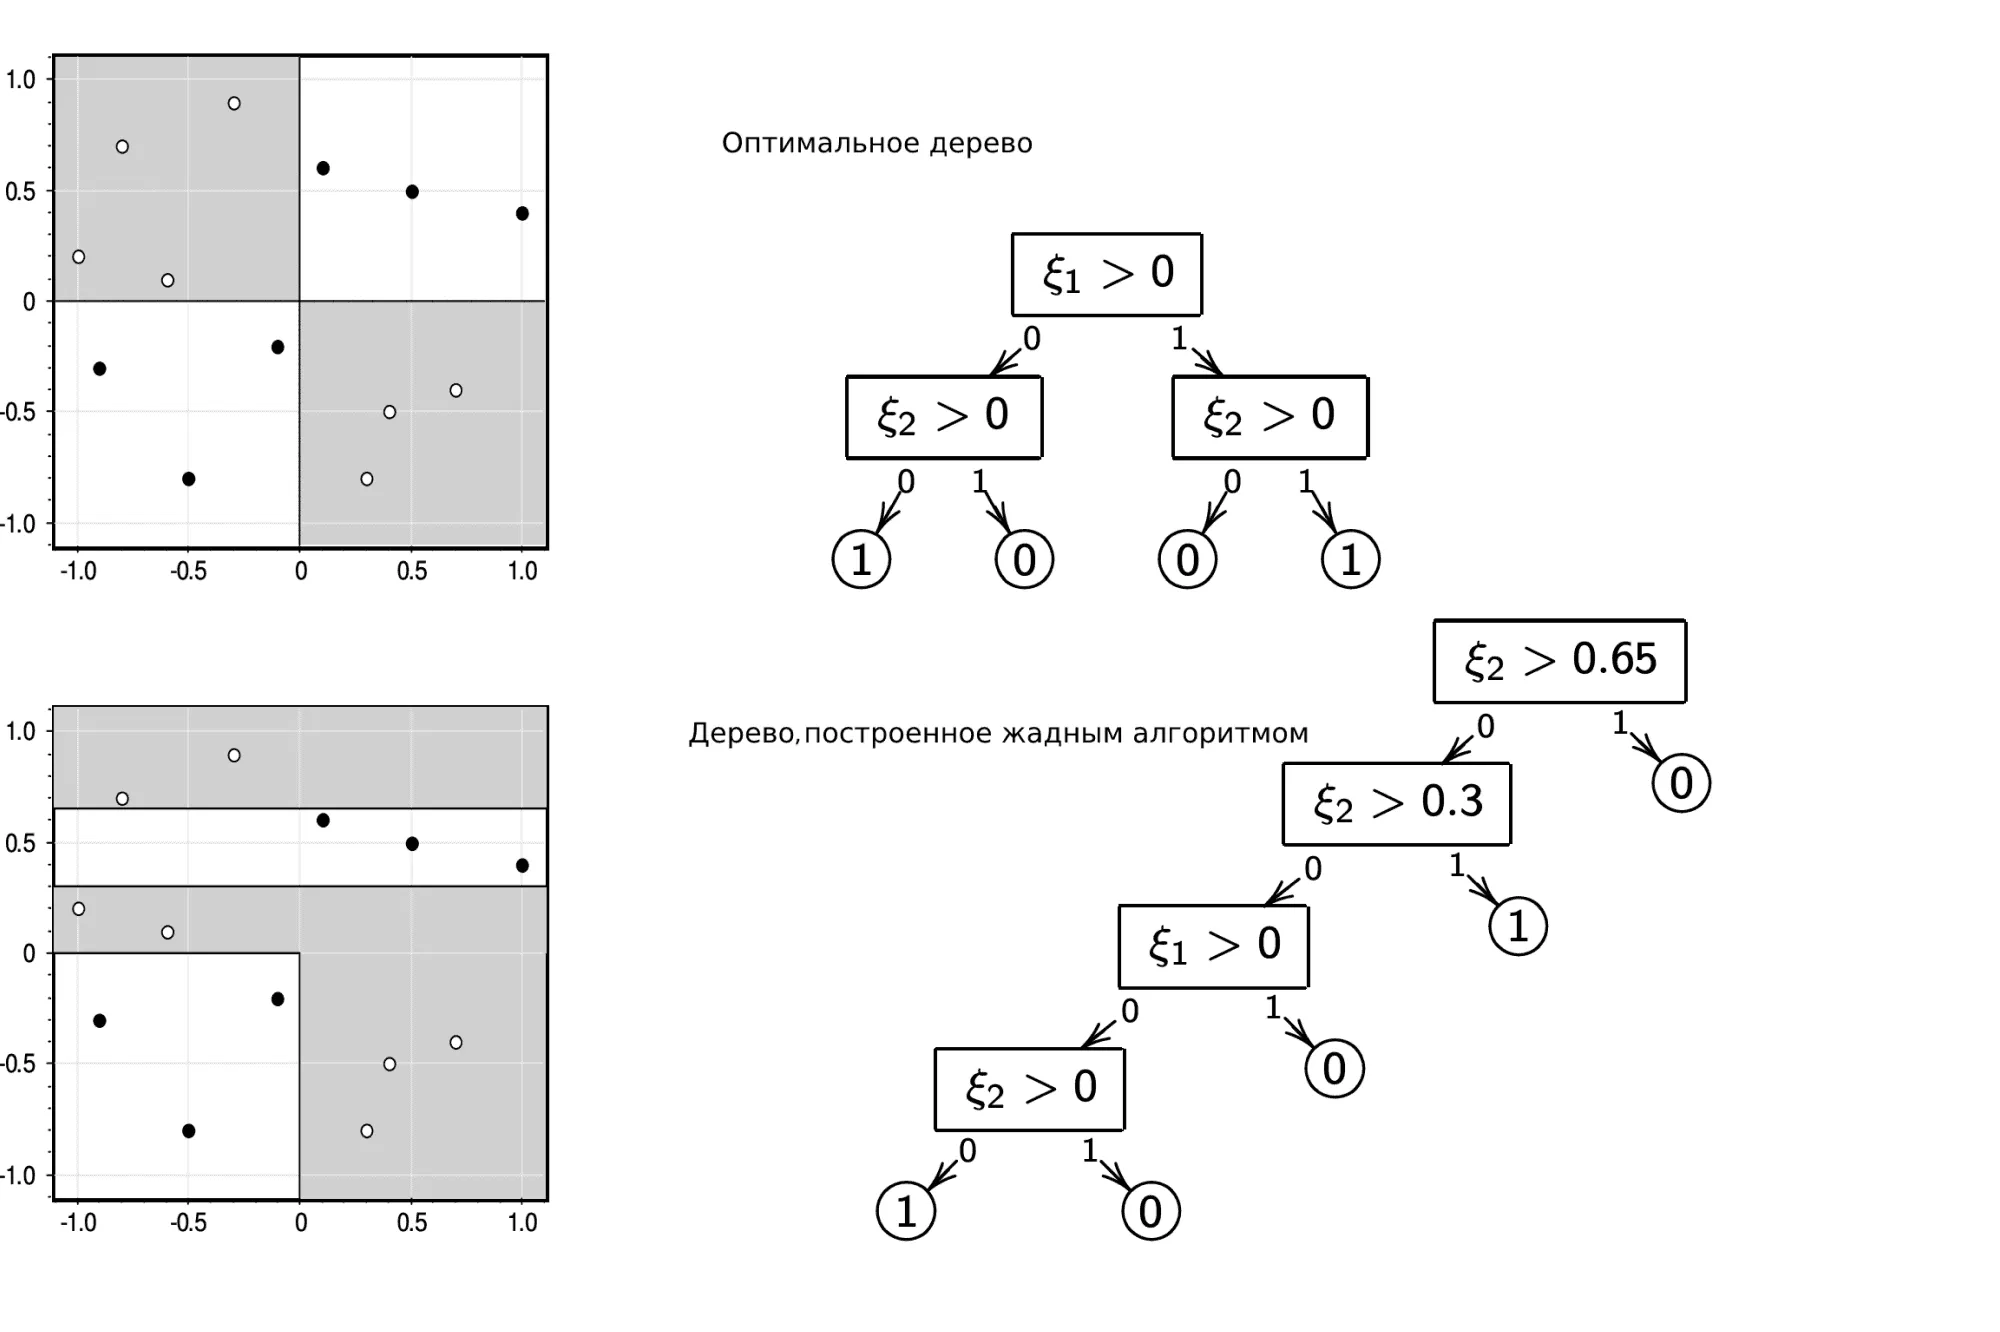
\includegraphics[width=1\textwidth]{not_optimal}
	\end{frame}
	
	\begin{frame}
		\frametitle{Листовые вершини}

		Пусть выполен критерий остановки и необходимо выбрать ответ для данного листа $Ans(X_m)$.

		\vspace{15pt}

		Можно выбирать из следующих соображений:
		\begin{itemize}
			\item Классификации --- метка наиболее частого класса, или можно оценить вероятности классов по
			частотам.
			\item Регрессия --- среднее, медиана или другая статистика.
			\item Простая модель, например для объктов дошедших до текущего листа выдавать ответ модели, обученной на
			соответсвующей подвыборке.
		\end{itemize}
	\end{frame}

	\begin{frame}
		\frametitle{Критерий остановки}

		В качестве критерия остановки можно взять:

		\begin{itemize}
			\item Объекты в вершине принадлежат одному классу или достаточно однородны
			\item Объектов в вершине слишком мало
			\item Неудается подобрать удачное разбиение $X = X_L \cup X_R$
		\end{itemize}
	\end{frame}

	\begin{frame}
		\frametitle{Критерий ветвления}

		Как определить оптимальное разбиение здесь и сейчас? Имеем на вход подвыборку $X_m$

		Пусть задача функция ошибки $L(y, c)$ 

		\vspace{15pt}
		
		Если текущую вершину сделать листовой и подобрать $c$, то достиигнем минимальной средней ошибки

		\[
		H(X_m) = \min_{c \in Y} \frac{1}{|X_m|} \sum_{i=1}^{m} L(y_i, c)
		\]

		Величину $H$ называют \textbf{информативностью} (impurity).
	\end{frame}

	\begin{frame}
		\frametitle{После разбиения}

		Быть может сможем разбить $X_m = X_L \cup X_R$  используя предикат~$b$ и решить в каждой новой вершине задачу отдельно.

		\vspace{15pt}

		Средняя ошибка после разбиения
		\[
		\frac{1}{|X_m|} \left( \sum_{x \in X_L} L(y_i, c_L) + \sum_{x \in X_R} L(y_i, c_R) \right)
		=
		\]
		\[
		= \frac{|X_L|}{|X_m|} H(X_L) + \frac{|X_R|}{|X_m|} H(X_R)
		\]
	\end{frame}

	\begin{frame}
		\frametitle{Прирост информативности}

		Рассмотрим разность информативности до разбиения и после

		\[
		IGain(b, X_m) = H(X_m) - \frac{|X_L|}{|X_m|} H(X_L) + \frac{|X_R|}{|X_m|} H(X_R)
		\]

		Если значение велико, значит нам выгодно произвести такое разбиение. Кроме того,
		чем больше --- тем лучше. 

		\vspace{15pt}

		Предикат $b$ при котором достигается наибольшее значение $IGain$ и выбирается для текущей вершины.
	\end{frame}

	\subsection{Критерии информативности}

	\begin{frame}
		\frametitle{Энтропия}

		Энтропия --- мера неопределенности распеделения

		\[
		H(X_m) = - \sum_{k=1}^{K} p_k \ln p_k
		\]

		\begin{itemize}
			\item Энтропия равна нулю у тривиальной случайной величине (принимает одно значение)
			\item Наибольшее значение энетропии у равномерного распределения.
		\end{itemize}
	\end{frame}

	\begin{frame}
		\frametitle{Критерий Джини}
		Также используется критерий Джини.

		\[
		H(X_m) = \sum_{k=1}^{K} p_k (1 - p_k)
		\]

		$H(X_m)$ равно математическому ожиданию числа неправильно классифицированных объектов в случае, 
		если мы будем приписывать им случайные метки из дискретного распределения, заданного вероятностями
		$(p_1, \dots, p_k)$
	\end{frame}

	\section{Обработка пропусков}

	\begin{frame}

	\end{frame}

	\section{Регуляризация деревьев}

	\begin{frame}
		
	\end{frame}
\end{document}
